\chapter{Related Work and Foundation}
\label{chap:relatedWork&Foundation}

The research on data visualization was settled in the context of Power Plants and their production mapping based on the geographical information system.  This chapter discusses related work about interactive maps and time series visualization. 

\section{Interactive Maps}

Maps are one of the more popular ways in visualizing geolocated data. There exist many web based dynamic interactive maps to visualize large, complex and compressed data sets with the powerful interface. These are used to present economical, cultural, or scientific information about different geographical objects or locations such as cities, districts, or countries. It requires less search time to find objects and locations of interest than a non-interactive map. These interactive maps are equipped with a variety of features and glyphs to simplify visual comparison and to speed up the search among displayed entities. Nowadays maps are light weight and portable. Unlike old techniques, new generation maps provide users an environment where the user can manipulate the data by clicking, scrolling, zooming, and get the details on demand. Color mapping, transparency, and glyphs allow guiding users in an understandable way to grasp information from the whole context of visualization of a large data set, which is presented on the display. Modern interactive maps additionally allow filtering techniques and retrieving information in an efficient manner. This flexibility of modern technique is attained by providing a clear and concise UI.

In September 2016, CarbonBrief \cite{cbg2016} has published an interactive map on their official website with an article named "How Germany generates its electricity". This is built using two open source libraries "Leaflet" and "Mapbox" which illustrates all renewable and non-renewable power plants inside Germany. This map depends on information distributed by the German Federal Network Agency. A circle area marker is used to locate the power plants and its area represents the capacity, as shows in the Figure \ref{fig:mapcb}. Unfortunately, the vast majority of the power plant areas depend on postcodes which are changed over to degrees latitude and longitude. Therefore, their location is not accurate. Within this map, a drop-down selector is used for interaction. Users can filter data on the map by selecting different power sources. An unique color is used for each source. But its significance is not explained in the online article.

\begin{figure}
  \begin{center}
    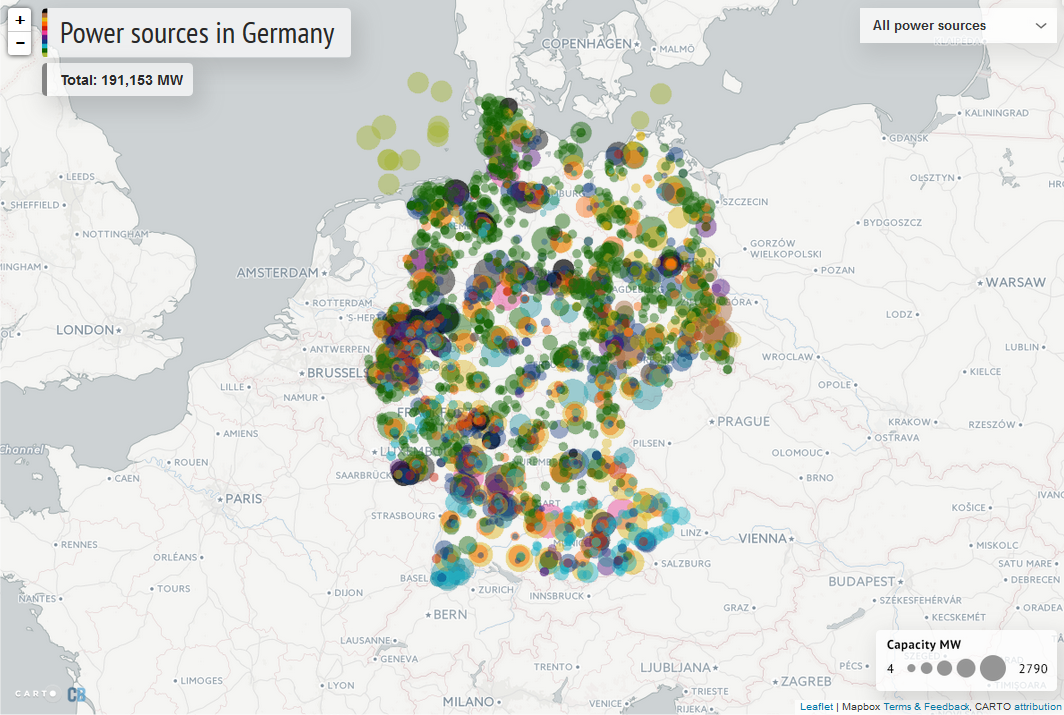
\includegraphics[width=1\textwidth]{mapcb}
    \caption{Interactive map showing the electricity production of Germany}
    \label{fig:mapcb}
  \end{center}
\end{figure}

Another interesting approach to the interactive map was published on July 2015 in the Washington Post \cite{wp2015} under the article of "How United states generate its electricity". This map provides information available power sources and its capacity in MW per US state. Like the previous example, circular area marker is also used here to locate power plants. Unfortunately, its not possible to know the capacity of each source individually. A Choropleth map is used to render different states inside the USA. The user can get information about the total power generated in a state by hovering over any state inside the map. The details of Choropleth map is discussed later in this section. A label is bound to each state which shows the total power generated by each source category and the area of the state is filled with darker color according to the principle of choropleth map. Unlike the previous example, no additional control layers are provided along with the map which makes it less interactive. However, meaningful and self explanatory glyph are used to define each power plants. The color of the logo of a power plant and color of the circular marker of the same power plant is the same. This scheme makes it easier to focus on each power plant category from a large dense area of the map.

\begin{figure}
  \begin{center}
    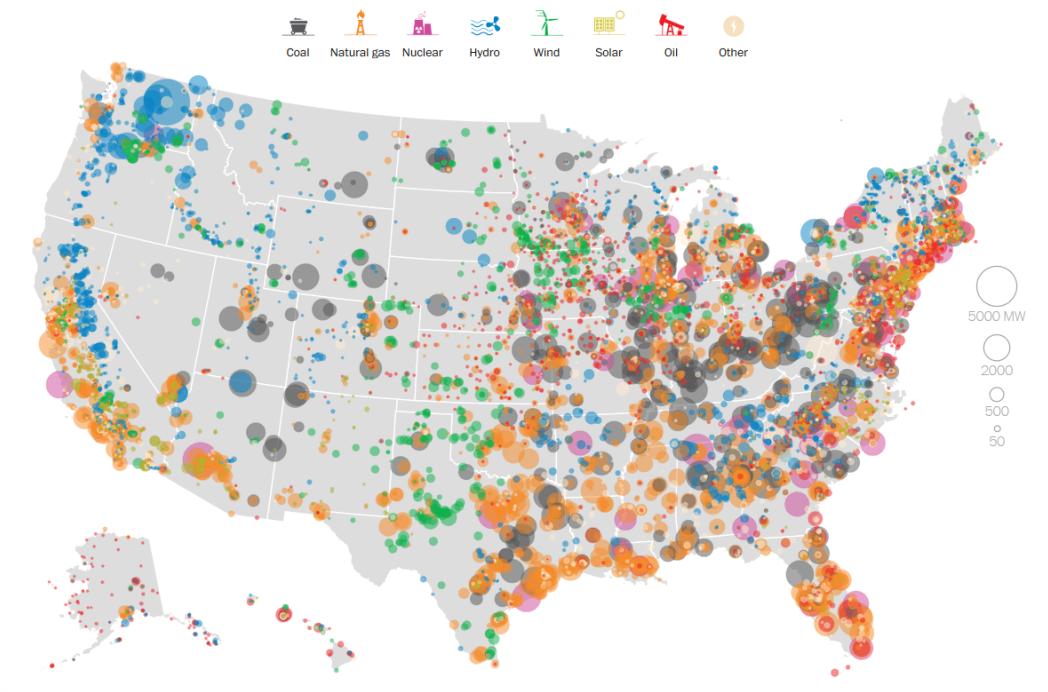
\includegraphics[width=1\textwidth]{mapusa}
    \caption{Interactive map showing how the United States generates its electricity}
    \label{fig:mapusa}
  \end{center}
\end{figure}

Choropleth map, Propotional Symbol map, Pinpoint maps, Connection maps, Isopleth maps are common types. In our case, particularly Pinpoint map and Choropleth are focused for locating the power plants and visualize their density inside Germany. In general, Choropleth Map displays geographical area surrounded by the border or area is colored or shaded in relation to a data variable. This mapping techniques provide a way to visualize density/value over an area. A color progression scale is used to represent the value in each area. On the other hand, pinpoint mapping is used to visualize the exact location of things. Currently, this mapping technique has become more popular. For example, Google Maps show the exact locations of points of interest. Companies from different sectors and service providers are creating their own applications using Google Maps or OpenStreetMap to share locations of different places such as banks, ATM machines, restaurants, hospitals, shopping malls, roads, rail ways, and shortest paths. We have used this mapping technique to visualize the exact geographical location of the power plants in Germany.

\subsection{Visualization Techniques}

\subsection*{Glyph-Based Visualization}

In different approach for locating renewable and non-renewable power plants and their production 
different countries have adapted different approaches. A common technique that has been observed from research, such as \cite{cbg2016} and \cite{wp2015}, is a circular area on the map. Circular area is the most used marker on the map. Basically, the center of the circle is locating the position and its area is describing the electricity production capacity of that corresponding power plant. These circular areas are filled with colors to categorize the power plants. Circles filled with different colors are easy to identify without deep investigation. To visualize the capacity along with the location of the power plant an ordinal data type is used to compare the size of a circle which is relative to a certain amount of Gigawatts or Megawatts. Mostly a legend is added to the map which provides useful meaning about the circles and helps the user to perceive useful information from the map. On the other hand symbols or glyph are used to represent the object which is the most fundamental way to show the position of power plants on the map. Markers with different colors are also used for easier navigation. Essentially markers can be used to represent anything that has a global position in latitude and longitude coordinates. Every interactive map generation tool provides default markers, which are familiar to most users. However, developers are able to change the markers or add own meaningful marker images. Along with the marker additional label or snippet added to provide more information or description about the marker. This title or snippet is displayed in an info window, a bubble appears over the marker when the user clicks or hovers over the marker.

CarbonBrief \cite{cbg2016} and the Washington Post \cite{gportal2016} have introduced two interactive maps. They provide information on how Germany generates its electricity. Both maps have used a colorful circular marker to locate the position of the plant inside Germany as well as the area of the circle representing the capacity. An internal drop-down navigation menu is added to the map of \cite{cbg2016} where the user can filter the plants by selecting different sources from the menu. On the other hand, \cite{gportal2016} is showing 380kV and 220kV power lines inside Germany along with the circular marker locating the plants and their generation. But there are no menu selection mechanism or filters for showing different power plants on the map. The available interaction techniques might be difficult for the users who are not expert enough using this type of interactive visualization tools. 

However, those approaches are missing the opportunity to engage user into the map on initial view. Circular markers with different colors might confuse the users to interpret the specific type of power plants. In particular, there is more than one unit of power plants are located in the same area. A plant with smaller generation capacity can be overlapped by a plant with larger capacity because of of its larger circular area. Therefore, pin point marker is used in our visualization framework to locate the power plants on the map. Logo inside the marker is self-explanatory and color of the markers is provided by the data set.
 
\subsection*{Interface and Interaction}

In CarbonBrief \cite{cbg2016} a full width map is used with menu selection mechanism (Figure \ref{fig:mapcbm}). With this menu selection, the user can select different categories of power sources. All this menu are hidden in the drop down section. Users are able to select only one category at a time from the menu. There is no possibility to select multiple categories of sources and render them into the map. This restricts users to view their desired power plants on the map. On the other hand, the Washington Post in \cite{wp2015} has published the map with not much functionality. No additional navigation menu is provided along with the map. To get details, user needs to hover over the map.

\begin{figure}
  \begin{center}
    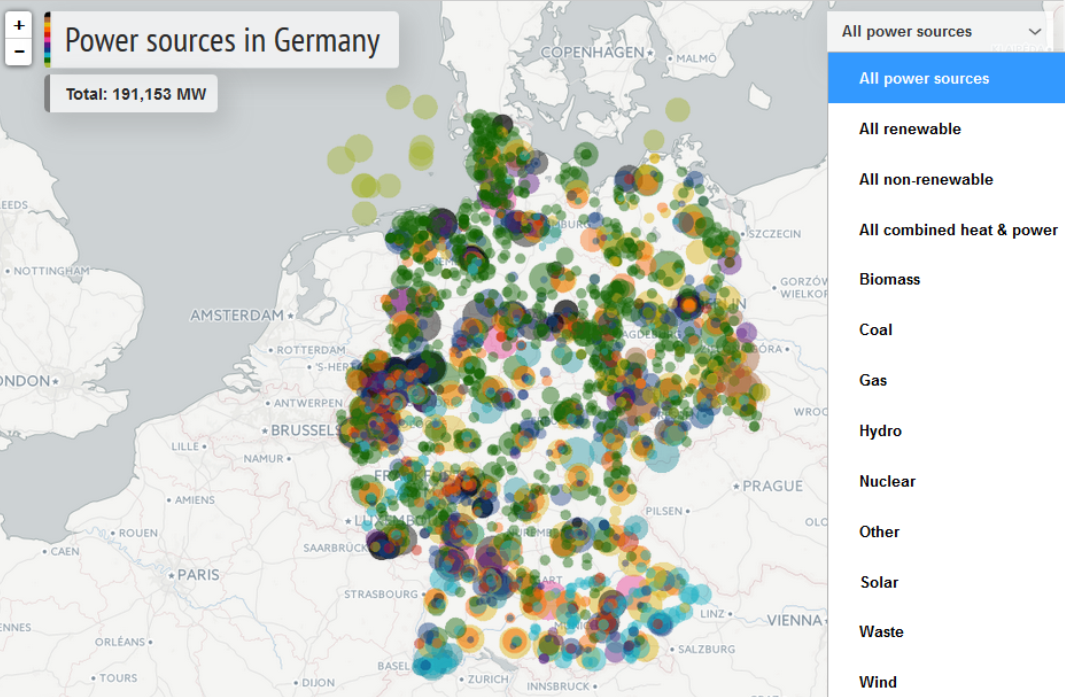
\includegraphics[width=1\textwidth]{mapcbddm}
    \caption{Interactive map : Menu selection mechanism}
    \label{fig:mapcbm}
  \end{center}
\end{figure}

In Geoportal \cite{gportal2016} also published a web based interactive map and providing information with a large and complex interface. Their interactive map has multiple functionality but still, lacks some important features.  For example, they are visualizing the power plants, which has the capacity above 100MW or equal as we are doing with our visualization framework. But there is no scope of power plant selection mechanism (Figure \ref{fig:mapgeo}).   
A descriptive but rather complex legend is added on the map. The user might find it difficult and it would take more time to explore the desired output out of this information visualization technique.

\begin{figure} [H]
  \begin{center}
    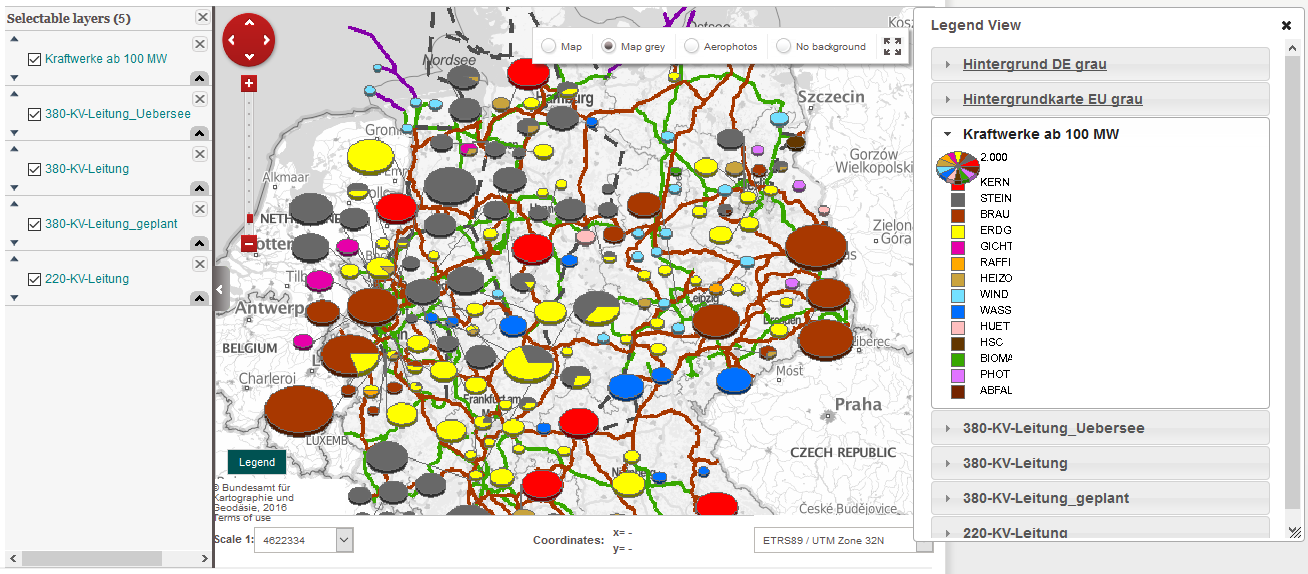
\includegraphics[width=1\textwidth]{geomapcl}
    \caption{Interactive map with Selectable layers and Legend.}
    \label{fig:mapgeo}
  \end{center}
\end{figure}

All these approaches and visualization techniques indeed enable users to extract the desired information from the map. However, in our visualization tool, we tried to make a clear, concise and efficient user interface. It might be easier for the user to figure out how our application works. We also tried to use familiar and consistent approaches to make the interface intuitive and given some more functionality to the users which are somehow missing in \cite{cbg2016}, \cite{wp2015} and \cite{gportal2016}. 

\section{Time Series Visualization}

There are countless visualization techniques that show time series data in the charts. One of the unique time series visualization is ThemeRiver \cite{981848} or Stacked Area Chart. This visualization depicts the thematic variations and changes over time within a large collection of data. The changes are shown in the context of a time line. The main focus of this visualization is to allow users to discern patterns which help to understand trends of the data-set. The theme river flow is directed from left to right. The variation of width represents the variation in the degree of representation unit. The horizontal width between two points on the theme river represents time interval and vertical distance or height of the river at any point of time indicates the strength of that point of the corresponding data set. It shows several streams, i.e. variables which changes over time and lays on top of each other as a layer. In visualization methods for time dependent data, Mueller and Schauman in \cite{1261490} have discussed different conventional approaches for visualizing time dependent data. ThemeRiver is one of the most well-known techniques to visualize multivariate data over Time. An intuitive interpretation of temporal changes can be observed by using this technique. In February 2008 New York Times depicted the “Ebb and Flow of Movies: Box Office Receipts Over Past 20 Years” \cite{boxoffice} (see Figure \ref{fig:nyk}). It was an interactive ThemeRiver visualization which illustrates the pattern of the amount of money films over a 21 years period make at the box office. This total figure is shown by varying heights and widths that reach over time. A color scale is used to reveal the amount of revenue range. The online response to this visualization was drastic and controversial. Marco and Yifan also mention in \cite{CGF12910} about this New York Times(NYT) publication. Later Byron and Wattenberg \cite{Byron2008} outlined three issues which affected the aesthetics of the graph, e.g, the ordering different layers, the shape of the lowest curve, which suppose to be the baseline and the labels of the layers. ThemeRiver fits in a general mathematical framework. A standard way to visualize time series data is to plot them on a Cartesian graph, which has time on the x-axis and the numeric values on the y-axis. A flat baseline allows the user to easily read the total diagram. 

\begin{figure}
  \begin{center}
    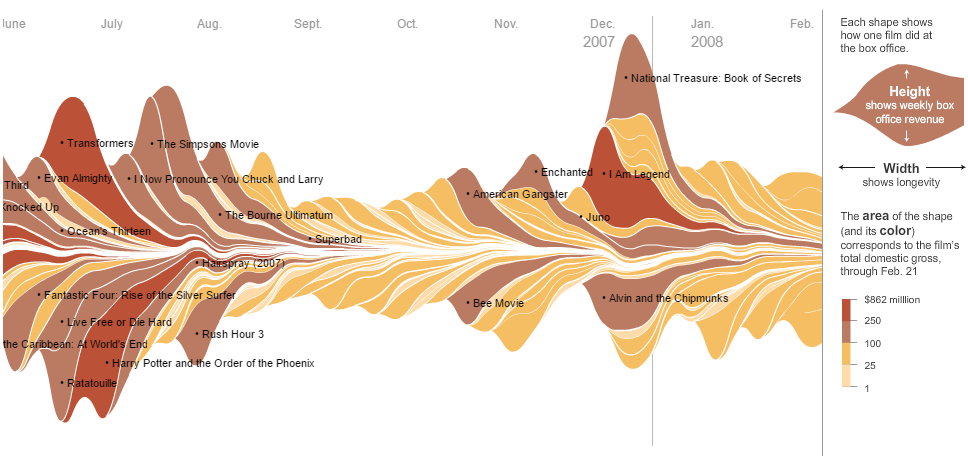
\includegraphics[width=1\textwidth]{nyt}
    \caption{Ebb and Flow of Movies: Box Office Receipts Over Past 20 Years visualized using ThemeRiver. Source:\cite{boxoffice}}
    \label{fig:nyk}
  \end{center}
\end{figure}

Later on, this flat baseline strategy has become very popular to visualize power production from renewable and non-renewable energy sources. Over time this visualization technology has been widely used. In another article of CarbonBrief \cite{cbuk2016}, ThemeRiver visualization technique (see Figure \ref{fig:ukecg}) is used to illustrate how UK is generating electricity over the last 50 years. Around 30\% of the UK electricity came from coal, which is clearly visibile from the illustration. On the other hand, US energy information administration in their Annual Energy Outlook 2017 \cite{eiagov} this flat base ThemeRiver is used to visualize the data for different aspects. Figure \ref{fig:eiatrgh} illustrates an example of it. 

\begin{figure}
  \begin{center}
    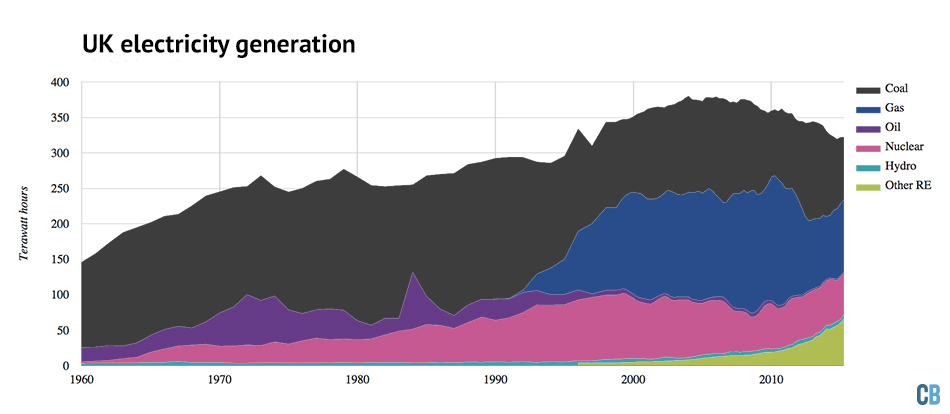
\includegraphics[width=1\textwidth]{UK-electricity-generation}
    \caption{UK electricity generation over time is visualized in the form of ThemeRiver (or Stacked Area Chart). Source:\cite{cbuk2016}}
    \label{fig:ukecg}
  \end{center}
\end{figure}

\begin{figure} [H]
  \begin{center}
    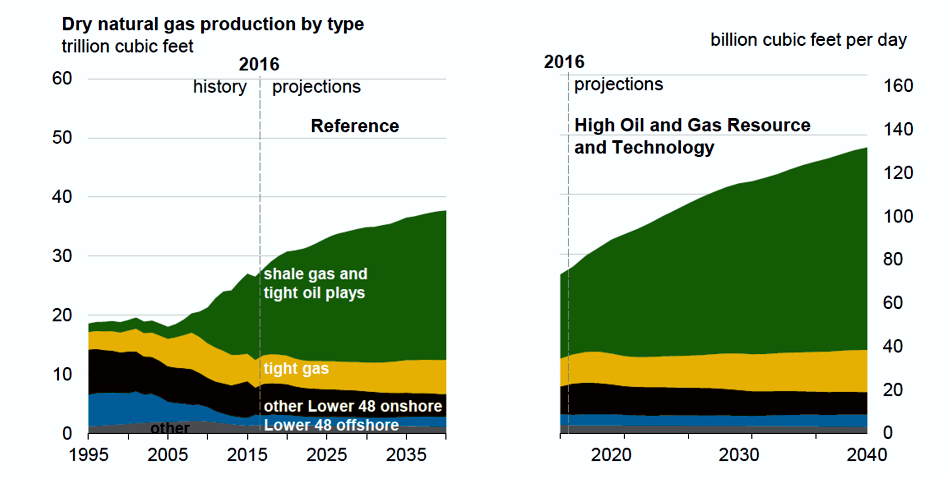
\includegraphics[width=1\textwidth]{eiatrg}
    \caption{U.S Dry natural gas production and future prediction over time is visualized in the form of ThemeRiver (or Stacked Area Chart). Source:\cite{eiagov}}
    \label{fig:eiatrgh}
  \end{center}
\end{figure}



